%%%%% Please set the path to 'beamer' directory in your environment %%%%%
\newcommand{\beamerDir}[0]{/mnt/c/Users/atsushi/Documents/workspace/env/Beamer/beamer/beamer/}


%%%%% Load setting %%%%%
\documentclass[aspectratio=169, dvipdfmx, 12pt, compress]{beamer}% dvipdfmxしたい

%%%%% Packages %%%%%
\usepackage{bxdpx-beamer}% dvipdfmxなので必要
\usepackage{pxjahyper}% 日本語で'しおり'したい
\usepackage{tikz}
\usepackage{tcolorbox}
\usetikzlibrary{shapes}
\usepackage{xcolor}
\usepackage[absolute,overlay]{textpos}
\usepackage{adjustbox}
\usepackage{caption}
\usepackage{ifthen}


%%%%% Settings %%%%%
\usetheme[sectionpage=progressbar, subsectionpage=progressbar]{metropolis}
% block style
\metroset{block=fill}
% space between line
\renewcommand{\baselinestretch}{1.3}
% space between item
\newlength{\wideitemsep}
\setlength{\wideitemsep}{0.9\itemsep}
% \addtolength{\wideitemsep}{1.0pt} <- more space
\let\olditem\item
\renewcommand{\item}{\setlength{\itemsep}{\wideitemsep}\olditem}
% frame title
\definecolor{coolblack}{rgb}{0.0, 0.18, 0.39}
\setbeamercolor{frametitle}{bg=coolblack!90,fg=white}
\setbeamerfont{frametitle}{size=\large}
\addtobeamertemplate{frametitle}{}{\vspace{-1em}}
\makeatletter
\setlength{\metropolis@frametitle@padding}{1.4ex}% <- default 2.2 ex
% foot line
\addtobeamertemplate{footline}{}{\vspace{-1em}}
% normal text color
\setbeamercolor{normal text}{fg=black!80}
% progress bar
\definecolor{lightgray}{rgb}{0.83, 0.83, 0.83}
\setbeamercolor{progress bar}{bg=lightgray, fg=coolblack}
\setbeamersize{text margin left=15pt, text margin right=15pt}
% equation font
\usefonttheme{professionalfonts}
% Change standard block width
\addtobeamertemplate{block begin}{%
    \centering
    \begin{columns}\begin{column}{0.9\textwidth}
            \centering
            }{}
            \addtobeamertemplate{block end}{}{\end{column}\end{columns}}
% Change alert block width
\addtobeamertemplate{block alerted begin}{%
    \centering
    \begin{columns}\begin{column}{0.9\textwidth}
            \centering
            }{}
            \addtobeamertemplate{block alerted end}{}{\end{column}\end{columns}}
% Change example block width
\addtobeamertemplate{block example begin}{%
    \centering
    \begin{columns}\begin{column}{0.9\textwidth}
            \centering
            }{}
            \addtobeamertemplate{block example end}{}{\end{column}\end{columns}}
% Itemize color
\setbeamertemplate{itemize item}{\color{black}\scriptsize$\blacksquare$}
\setbeamertemplate{itemize subitem}{\color{black}\scriptsize$-$}
% Simplification  color
\definecolor{cobalt}{rgb}{0.0, 0.28, 0.67}
\setbeamercolor{block title example}{fg=black!80,bg=cobalt!35}
\setbeamercolor{block body example}{fg=black,bg=cobalt!15}
% Definition
\BeforeBeginEnvironment{definition}{
    \setbeamercolor{block title}{use=alerted text, bg=alerted text.fg!70,fg=white}
    \setbeamercolor{block body}{use=alerted text, bg=alerted text.fg!20}
}
\AfterEndEnvironment{definition}{% return to default
    \setbeamercolor{block title}{use=structure,fg=structure.fg,bg=structure.fg!20!bg}
    \setbeamercolor{block body}{parent=normal text,use=block title,bg=block title.bg!50!bg, fg=black}
}
% Theorem
\definecolor{seagreen}{rgb}{0.18, 0.55, 0.34}
\setbeamertemplate{theorems}[numbered]
\BeforeBeginEnvironment{theorem}{
    \setbeamercolor{block title}{fg=black!80,bg=seagreen!40}
    \setbeamercolor{block body}{fg=black,bg=seagreen!15}
}
\AfterEndEnvironment{theorem}{% return to default
    \setbeamercolor{block title}{use=structure,fg=structure.fg,bg=structure.fg!20!bg}
    \setbeamercolor{block body}{parent=normal text,use=block title,bg=block title.bg!50!bg, fg=black}
}
% Lemma
\undef{\lemma}
\newtheorem{lemma}{\translate{Lemma}}
\BeforeBeginEnvironment{lemma}{
    \setbeamercolor{block title}{fg=black!80,bg=seagreen!20}
    \setbeamercolor{block body}{fg=black,bg=seagreen!10}
}
\AfterEndEnvironment{lemma}{% return to default
    \setbeamercolor{block title}{use=structure,fg=structure.fg!80,bg=structure.fg!20!bg}
    \setbeamercolor{block body}{parent=normal text,use=block title,bg=block title.bg!50!bg, fg=black}
}


%%%%% Original Command %%%%%
\newcommand{\subt}[1]{\vspace{-2mm}{\fontsize{10pt}{0cm}\selectfont \textcolor{lightgray}{#1}}\vspace{-1mm}}
\newcommand{\lastpage}[0]{\begin{frame}\begin{textblock*}{1.0\linewidth}(0pt, 50pt)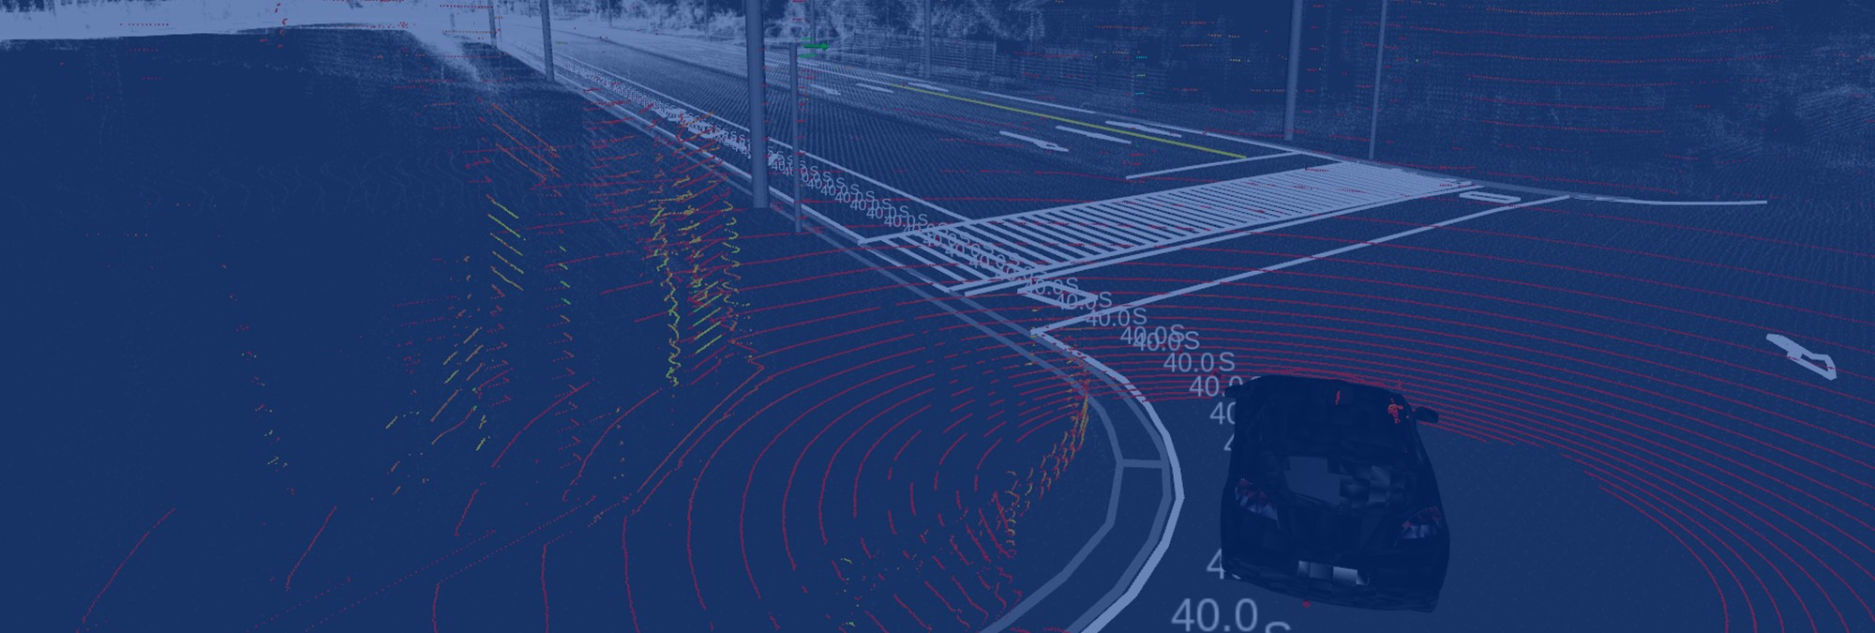
\includegraphics[scale=0.512]{\beamerDir/master_figure/last.pdf}\end{textblock*}\end{frame}}
\newcommand{\todo}[1]{\al{\LARGE\textbf{TODO:} #1}}
\newcommand{\headerheight}[0]{5mm}
\newcommand{\footerheight}[0]{5mm}
\newcommand{\slideheight}[0]{\textheight-\headerheight-\footerheight}
\newcommand{\tabml}[1]{\hspace{-2.1mm}\begin{tabular}{l} #1 \end{tabular}}
\newcommand{\al}[1]{\alert{#1}}
\newcommand{\argempty}[0]{}
\newcommand{\onlyslide}[1]{
    \vspace{\headerheight}
    \begin{minipage}[c][\slideheight][c]{\textwidth}
        #1
    \end{minipage}
}
\newcommand{\onlyimage}[1]{
    \onlyslide{
        \centering
        \begin{columns}
            \begin{column}{\textwidth}
                \centering
                \adjustbox{max width=\textwidth, max height=\slideheight}{
                    \includegraphics{#1}
                }
            \end{column}
        \end{columns}
    }
}
% fit image
\newlength\fitimageht
\newlength\fitotherht
\newsavebox\fitimagebox
\newcommand{\fitimage}[2]{%
    \sbox\fitimagebox{%
        \parbox{\textwidth}{%
            #1\par
        }%
    }%
    \settototalheight{\fitotherht}{%
        \usebox\fitimagebox
    }%
    \setlength\fitimageht{\textheight}%
    \addtolength\fitimageht{-\fitotherht-\headerheight-\footerheight-1\baselineskip}%
    \vspace{\headerheight}
    #1\par
    \centering
    \includegraphics[width=\textwidth,height=\fitimageht,keepaspectratio]{#2}
}
% Simplification
\newcommand{\assume}[1]{
    \begin{exampleblock}{Simplification }
        #1
    \end{exampleblock}
}
% Re-post
\setbeamercolor{RepostBox}{fg=black!50, bg=coolblack!10}
\newcommand{\repost}[1]{
    \vspace{2mm}
    \centering
    \begin{columns}
        \begin{column}{0.86\textwidth}
            \begin{beamercolorbox}[wd=\textwidth, sep=2pt, rounded=true, shadow=true]{RepostBox}
                \begin{tabular}{|p{0.95\textwidth}}
                    {\fontsize{10pt}{10pt}#1}
                \end{tabular}
            \end{beamercolorbox}
        \end{column}
    \end{columns}
}

% equation ballon
\tcbset{
    framebox/.style={
            enhanced,
            boxsep=0pt,       % 箱の上下左右の余白を指定
            colback=white,
            boxrule=1pt,
            colframe=#1
        },
    framebox/.default=red
}
\newcommand{\upbln}[3]{
    \tcboxmath[
        framebox=#2,
        top=0.5ex,bottom=0.5ex,    % 箱の上下の余白を指定
        left=0.5ex,right=0.5ex,    % 箱の左右の余白を指定
        overlay={
                \node[
                    above,
                    rectangle callout,                         % nodeを吹き出しの形に
                    callout absolute pointer={(frame.north)},  % 吹き出しの先端を絶対的に指定
                    fill=#2!20
                ] at ([yshift=2ex]frame.north) {\footnotesize#3};
            }
    ]{#1}
}
\newcommand{\lwbln}[3]{
    \tcboxmath[
        framebox=#2,
        top=0.5ex,bottom=0.5ex,    % 箱の上下の余白を指定
        left=0.5ex,right=0.5ex,    % 箱の左右の余白を指定
        overlay={
                \node[
                    below,
                    rectangle callout,                         % nodeを吹き出しの形に
                    callout absolute pointer={(frame.south)},  % 吹き出しの先端を絶対的に指定
                    fill=#2!20
                ] at ([yshift=-2ex]frame.south) {\footnotesize#3};
            }
    ]{#1}
}
\tcbuselibrary{theorems,skins}



%%%%% Mode %%%%%
% \newcommand{\forme}[1]{#1}
\newcommand{\forme}[1]{}


%%%%% Front Cover %%%%%
\title{Virtually-Federated Scheduling of Parallel Real-Time Tasks}
\subtitle{IEEE Real-Time Systems Symposium (RTSS), 2021}
\author{矢野 篤志}
\date{\today}
\institute[EMBIV]{EMBIV}
\logo{\begin{textblock*}{0.1\linewidth}(2pt, 237pt)
\includegraphics[scale=0.4]{\beamerDir/master_figure/Emb_logo.pdf}\end{textblock*}}


%%%%% Document Start %%%%%
\begin{document}

\maketitle

% \summary{3}{0}
% !TeX root = main.tex


\begin{frame}{提案の概要}
    \begin{itemize}
        \item 優先度駆動型スケジューリングによってROSのリアルタイム性能と予測可能性を大幅に改善できることを主張する
        \item 主張を裏付けるために, 優先度駆動型チェーン考慮スケジューリングに関する我々の研究をレビューし, Apex.AI が開発したオープンソースリファレンスシステムを用いた評価を行う
        \item ROS 2のリアルタイム性能を向上させるために不可欠な以下2つの課題を説明する
        \begin{itemize}
            \item マルチスレッドエグゼキュータ設計
            \item アクセラレータサポート
        \end{itemize}
    \end{itemize}
\end{frame}


\begin{frame}{Outline}
    \setbeamertemplate{section in toc}[sections numbered]
    \scriptsize\tableofcontents[hideallsubsections]
\end{frame}

% % !TeX root = main.tex

\section{PRIOR KNOWLEDGE}
\label{sec: prior knowledge}

\begin{frame}{前提知識}
    \begin{itemize}
        \item \ourl{ROS}{https://tier4.atlassian.net/wiki/spaces/EMBIV/pages/2683603071/ROS+Robot+Operating+System}
        \item \ourl{publish/subscribeモデル}{https://tier4.atlassian.net/wiki/spaces/EMBIV/pages/2675048610/Publish+Subscribe}
        \item \ourl{SCHED\_DEADLINE}{https://tier4.atlassian.net/wiki/spaces/EMBIV/pages/2692645566/SCHED+DEADLINE}
        \item \ourl{最大イベント到着曲線}{https://drive.google.com/file/d/1n85X0vDrDm4IDANDP4aUoC0SNnZLAiRN/view?usp=share_link}
        \item \ourl{Casiniらによる先行研究}{https://drive.google.com/file/d/1sHujFqbmgCoJbC6g6KdC7ihua4Jqddju/view?usp=share_link}
    \end{itemize}
\end{frame}

% % !TeX root = main.tex

\section{INTRODUCTION}
\label{sec: introduction}

\begin{frame}{}
    \begin{itemize}
        \item ロボット工学のような, 様々な分野の深い専門知識を必要とする学際的で複雑なアプリケーション領域では, 通常, 全ての, あるいはほとんどのソフトウェアをゼロから書くという選択肢はあり得ない
        \item その代わりに, ロボット工学者は, ROSのような一般的なロボット工学フレームワークで容易に利用できる, 標準機能を提供する既存のサードパーティコンポーネントの統合を採用するのが一般的である
        \item その利点は数多く, 簡単に理解できる
        \item 例えば, 複数の最新パス計画アルゴリズムと3D可視化サポートを備えた完全なナビゲーションスタックがたった1回のダウンロードで手に入るなら, なぜ新しいナビゲーションサブシステムを苦労して開発する必要があるか?
    \end{itemize}
\end{frame}

\begin{frame}{}
    \begin{itemize}
        \item 完全なロボットシステムを構築するためには, 多くの相互作用するコンポーネントを統合する必要がある
        \item ROS開発プロセスの分散型オープンソースの性質により, これらのコンポーネントは通常, 必ずしもお互いを知らない複数の独立したコンポーネント開発者によって分離して開発される
        \item 同様に, システムインテグレータは, アプリケーションおよびミッション固有のロジックと「グルーコード」で展開プラットフォーム上で選択したコンポーネントを構成するが, 通常, それぞれのコンポーネント開発者と密接に連携することはない
    \end{itemize}
\end{frame}

\begin{frame}{}
    \begin{itemize}
        \item コンポーネントの統合を可能な限りシンプルに保つために, ROSはコンポーネントの疎結合を可能にする古典的なトピックベースのpublish/subscribeパラダイムを採用している
        \item 概念的には, 各コンポーネントは, 特定のトピックをsubscribeする多数のコールバックを含む「ブラックボックス」として理解できる
        \item 与えられたトピックに関連するメッセージがpublishされるたびに, 全てのsubscribeコールバックが呼び出され, 何らかの計算を実行し, 次に他のトピックに後続のメッセージをpublishすることができ, これがさらにコールバックをトリガするというように, 繰り返す
    \end{itemize}
\end{frame}

\begin{frame}{}
    \begin{itemize}
        \item インテグレータは, あるコンポーネントの「入力コールバック」を別のコンポーネントの「出力トピック」に接続することによってコンポーネントを構成する
        \item ROSシステムは, このように相互接続されたトピックとコールバックの複雑なネットワークを形成し, データ (環境刺激など) は, イベント駆動型の方法でネットワークを通じてcause-effectチェーンに沿って伝播し, インテグレータが望むように透過的にコンポーネント境界を交差させることができる
    \end{itemize}
\end{frame}

\begin{frame}{}
    \begin{itemize}
        \item このようなcause-effectチェーンの典型的な例として, 進路上の障害物を検知して反応する必要のある移動ロボットのセンシング-計算-行動パイプラインが挙げられる
        \item 例えば, ハードウェアドライバコンポーネントがレーザースキャナから新しいサンプルを取得し (cause) , それが複数のマッピング, 座標変換, パス計画, 車輪制御コンポーネントを経て, 最終的に車輪速度の変化 (effect) をもたらす可能性がある
        \item このようなデータ処理のチェーンにおいて, causeからeffectまでの最大レイテンシ時間は, ロボットが正しく機能するために重要な役割を果たすことは明らかであり, また, 安全性を考慮する上でも重要であることが多い
    \end{itemize}
\end{frame}

\begin{frame}{}
    \begin{itemize}
        \item 重要なのは, システムインテグレータにできるだけ多くの展開の選択肢を残し, コンポーネントの再利用の機会を最大化するために, ROSの実行管理層と基礎となるオペレーティングシステムは, 意図的にコンポーネント開発者に公開されないことである
        \item むしろ, ROSの中心的なコールバック抽象化は, コールバック手続きがいつどのようにスケジュールされるか, コールバックの実行がスレッドまたはプロセスにわたってどのように組織されるか, またはネットワーキング層がメッセージの送受信をどのように処理するかを全く意識せずに, 実行から完了までセマンティクスを持つ単なる手続きである
    \end{itemize}
\end{frame}

\begin{frame}{}
    \begin{itemize}
        \item ROSはオープンソースソフトウェアであるため, 原理的にはシステムの実行と通信の挙動を完全に理解し制御することが可能である
        \item このため, リアルタイムシステムの専門家から見れば, ROSにリアルタイムシステム研究でよく知られた技術を導入することは論理的なステップであるように思える可能性がある
        \item しかし, 一見したところ, これを難しくしているハードルがいくつかある
    \end{itemize}
\end{frame}

\begin{frame}{}
    \begin{itemize}
        \item まず第一に, インテグレータに必要な情報が不足している
        \item ほとんどのリアルタイム分析では, 同時実行タスクの数, それらの起動セマンティクスや機能的相互作用, メッセージの到着パターン, 最悪実行時間など, 多くの低レベルシステムの詳細に関する深い知識が前提となっている
        \item ROSコンポーネントは, この種の情報を提供するマニフェストと一緒に来ることはない
        \item さらに悪いことに, リアルタイム分析は, 欠陥のある情報や不完全な情報にうまく対処できない
        \item モデリング目的でサードパーティコンポーネントを手作業でリバースエンジニアリングしているときに, たった一つのミスや見落としがあれば, その取り組み全体を無条件に無効にしてしまうことになりかねない
    \end{itemize}
\end{frame}

\begin{frame}{}
    \begin{itemize}
        \item 第二に, 必要なシステムの詳細をコンポーネントレベルで静的に決定し, 記述することができない
        \item その理由のひとつは, 多くのロボット工学アルゴリズムが, ユースケースやプラットフォーム固有の側面に依存し, 実行時間や起動パターンが大きく変化するためである
        \item 例えば, ビデオストリーム中の物体を識別し, その軌跡を推測する一般的な物体追跡コンポーネントを考えてみよう (例えば, 隣の車線の車など)
        \item この機能の実行時間は, ビデオストリームのフレームレート, 解像度, コーデック, および特定のトラッキングアルゴリズムに関連する他の様々なパラメータを含む, 様々なパラメータに依存する
        \item これらのパラメータは, 一般的なオブジェクトトラッキングコンポーネントの開発者が前もって知っていたり, 固定されていたりするものではない
    \end{itemize}
\end{frame}

\begin{frame}{}
    \begin{itemize}
        \item このようなユースケース特有の情報は, 特定のロボットを構築するインテグレーターにしか分からない
        \item インテグレーターは, 必ずしもオブジェクトトラッキングやリアルタイムシステムの専門家ではないため, 特定の構成を選択した場合の影響を常に予測できるわけではない
        \item したがって, コンポーネントのリソース要求とリアルタイム動作は, 常に特定の展開で使用するという文脈で評価されなければならない
        \item これは, ROSフレームワークの人気の根底にある「ブラックボックス」コンポーネントのモジュール式再利用と相容れるものではない
    \end{itemize}
\end{frame}

\begin{frame}{}
    \begin{itemize}
        \item 最後に, 仮にインテグレータが各コンポーネントについてそれぞれの専門家と議論し, タイミング分析に必要な全ての詳細を入手できたとしても, 第三の根本的な問題が残る
        \item 多くのコンポーネントのリソース要件と性能特性は, 本質的にロボットの動的環境に依存し, したがって時間とともに変化するため, 静的 (最悪のケース) リソース配置は実行不可能なのである
    \end{itemize}
\end{frame}

\begin{frame}{}
    \begin{itemize}
        \item 例えば, 前述の物体追跡コンポーネントと, ランドマークベースの自己位置特定コンポーネントに依存するロボットを再度考えてみよう
        \item 一方, 人口が少ない田舎町よりも, にぎやかな街中を移動する方が, 物体追跡装置の処理時間はずっと長くなる
        \item 一方, 認識可能なランドマークが多い都市部では, ほぼ一様な風景よりも自己位置推定がはるかに容易である可能性が高い
        \item どちらの状況でも十分なリソースを確保するためには, システムインテグレーターは, 不毛の土地からなる賑やかな都市を想定したシステムを用意しなければならない
    \end{itemize}
\end{frame}

\begin{frame}{}
    \begin{itemize}
        \item ロボット工学では, このような悲観的なシステム設計を行うと, すぐに現実的な限界に直面することになる
        \item その代わりに, 実用的で費用対効果の高いシステムを維持するためには, 各コンポーネントのピーク需要の合計ではなく, 予想されるジョイントリソースのピーク需要に対してプロビジョニングを行う必要がある
    \end{itemize}
\end{frame}

\begin{frame}{貢献する}
    \begin{itemize}
        \item これらの課題を克服するために, 我々は, 実行時に動的にタイミングを考慮した方法でROSシステムをプロビジョニングするための自動レイテンシマネージャを使用することを提案する
        \item 具体的には, ROS Live latency manager (ROSLlama) を紹介する
        \item これは, 重要なcause-effectチェーンに沿ったレイテンシを, 非リアルタイム専門家が使いやすく, かつ設定にあまり手間をかけない方法で, 既存のリアルタイム機構を使用して制御することを可能にする
    \end{itemize}
\end{frame}

\begin{frame}{貢献する}
    \begin{itemize}
        \item ROS-Llamaは, 複雑なシステムパラメータをユーザに要求するのではなく, 実行時に必要なパラメータを自動的に推定し, 状況の変化に応じてスケジューリングパラメータを動的に調整することが可能である
        \item もし, 指定されたレイテンシの目標が全て同時に達成できない場合 (例えば, 不利な環境条件による一時的な過負荷が原因) , ROS-Llamaは制御された緩やかなデグレードプロセスを開始し, システムインテグレーターが純粋に宣言的な方法で (すなわち, cause-effectチェーンがどの部品を通過しているかを理解しなくても) cause-effectチェーンの重要性を特定できるようにする
    \end{itemize}
\end{frame}

\begin{frame}{本論文の貢献}
    \begin{itemize}
        \item  ロボティクス領域における動的レイテンシ管理問題を探求し, 実用的なソリューションが満たさなければならない制約と要件を文書化する (第III章)

        \item  ROSのための最初の自動レイテンシマネージャであるROS-Llamaの設計と実装を紹介する (セクションIV)

        \item 標準的な Linux システム上の ROS コンポーネントを用いて, ROS-Llama が移動ロボットのcause-effectチェーンのレイテンシをうまく制御できることを示す評価について報告する (セクションVI)

    \end{itemize}
\end{frame}

\begin{frame}{}
    \begin{itemize}
        \item ROS-Llamaは, 数年にわたる研究とエンジニアリングの努力の結果であり, その間, 我々は多くの課題や技術的な限界に遭遇した
        \item セクションVIIでは, 以下の点を強調する
              \begin{itemize}
                  \item  ROS-Llamaをより効果的かつ正確にするための分析改善の機会
                  \item  ROSとLinuxのプラットフォームには, システムのさらなる改良の妨げとなる大きな限界がある
              \end{itemize}
    \end{itemize}
\end{frame}

% !TeX root = main.tex

\section{SYSTEM MODEL}
\label{sec: system_model}


\begin{frame}{}
    以下では, 上記の説明から抽出したマルチスレッドエグゼキュータのリアルタイム関連の動作をカバーするスケジューリングモデルを紹介する
\end{frame}

\begin{frame}{}
    \assume{簡単にするために, wait\_set にアクセスまたは更新するスレッドによって発生するオーバヘッドはゼロであると仮定する}
\end{frame}

\begin{frame}{Notations1}
    \begin{table}[tb]
        \adjustbox{max width=\textwidth, max height=\slideheight}{
            \centering\begin{tabular}{|c|l|} \hline
                \textbf{Notations}      & \textbf{Descriptions}                                                                       \\\hline
                $C_i$                   & チェイン                                                                                    \\\hline
                $m$                     & スレッド数                                                                                  \\\hline
                $\Gamma $               & チェインのセット                                                                            \\\hline
                $c_{i,j}$               & $C_i$の$j$番目のコールバック                                                                \\\hline
                $e_{i,j}$               & $c_{i,j}$のWCET                                                                             \\\hline
                $E_i$                   & $C_i$内のコールバックのWCETの合計                                                           \\\hline
                $D_i$                   & $C_i$のデッドライン                                                                         \\\hline
                $T_i$                   & $C_i$の周期                                                                                 \\\hline
                % $U_i$                   & $C_i$の利用率                                                                               \\\hline
                % $\mathcal{G}(c_{i,j}) $ & $c_{i,j}$が属すmutually exclusiveコールバックグループのインデックス                         \\\hline
                $\theta_i$              & \tabml{$\mathcal{C}_{i}$ の各コールバックが属すmutually exclusiveコールバックグループの集合 \\ $\theta_{i}=\cup_{\forall c_{i, j} \in \mathcal{C}_{i}}\left\{\mathcal{G}\left(c_{i, j}\right)\right\}$} \\\hline
            \end{tabular}
        }
    \end{table}
\end{frame}

\begin{frame}{Notation2}
    \begin{table}[tb]
        \adjustbox{max width=\textwidth}{
            \centering\begin{tabular}{|c|l|} \hline
                \textbf{Notations} & \textbf{Descriptions}                                       \\\hline
                $J_{i}^{k}$        & $\mathcal{C}_{i}$ の $k$番目のインスタンス                  \\\hline
                $c_{i, j}^{k}$     & $J_{i}^{k}$ に含まれる$c_{i, j}$ のコールバックインスタンス \\\hline
            \end{tabular}
        }
    \end{table}
\end{frame}

\subsection{Workload Model}
\label{ssec: workload_model}

\begin{frame}{チェーンの定義}

    \begin{itemize}
        \item $m$ スレッド上のマルチスレッドエグゼキュータによってスケジュールされた一連の独立した処理チェーン (略してチェーンと呼ぶ) $\Gamma=\left\{\mathcal{C}_{1}, \mathcal{C}_{2}, \cdots, \mathcal{C}_{|\Gamma|}\right\}$ を検討する

              \assume{各スレッドは専用プロセッサに静的に展開されており,スレッドはいつでもプロセッサを使用できる}

        \item 各チェーン $\mathcal{C}_{i} \in \Gamma$ は, コールバック $\mathcal{C}_{i}=\left\{c_{i, 1}, c_{i, 2}, \cdots, c_{i,\left|\mathcal{C}_{i}\right|}\right\}$ の順序付けられたシーケンスで構成される
        \item $\mathcal{C}_{i}$ の最初のコールバック $c_{i, 1}$ (それぞれ, 最後のコールバック $c_{i,\left|\mathcal{C}_{i}\right|}$ ) は, $\mathcal{C}_{i}$ のソースコールバック (それぞれ, シンクコールバック) と呼ばれる
    \end{itemize}
\end{frame}

\begin{frame}{}
    \begin{itemize}
        \item 各コールバック $c_{i, j}$ は最悪実行時間 (WCET) $e_{i, j}$ によって特徴付けられる
        \item コールバックは, 固有のmutually exclusive コールバックグループまたはreentrant コールバックグループのいずれかに属している
    \end{itemize}
\end{frame}

\begin{frame}{}
    \begin{itemize}
        \item チェーン $\mathcal{C}_{i}$ は, チェーンインスタンスの無限シーケンスをリリースする
        \item $T_{i}$ の周期は, $\mathcal{C}_{i} \cdot \mathcal{C}_{i}$ の 2 つの連続するチェーンインスタンスのリリース時刻の間の最小間隔
        \item 相対デッドライン $D_{i}$ があり, 時間 $r$ でリリースされた $\mathcal{C}_{i}$ の各チェーンインスタンスは, その絶対デッドライン $r+D_{i}$ までに終了する必要がある
        \item チェーンには制約付きデッドライン, つまり $D_{i} \leq T_{i}$ があると想定している
        \item $\mathcal{C}_{i}$ の利用率は $U_{i}=E_{i} / T_{i}$ である
    \end{itemize}
\end{frame}

\begin{frame}{}
    \begin{itemize}
        \item $J_{i}^{k}$ 内の連続する要素 $c_{i, j}^{k}$ と $c_{i, j+1}^{k}$ の各ペアについて, $c_{i, j}^{k}$ を $c_{i, j+1}^{k}$ の先行要素, $c_{i, j+1}^{k}$ を $c_{i, j}^{k}$ の後続要素と呼ぶ
        \item 非シンクコールバックインスタンス $c_{i, j}^{k}$ が実行を終了すると, 後続のインスタンスを呼び出すメッセージが生成される
    \end{itemize}
\end{frame}

\begin{frame}{応答時間の定義}
    \begin{itemize}
        \item 応答時間 $R\left(J_{i}^{k}\right)$ は,  $J_{i}^{k}$ のリリース時刻と終了時間の間の時間間隔である
        \item チェーン $\mathcal{C}_{i}$ の最悪応答時間 $\mathcal{R}_{i}^{w c}$ は, そのすべてのインスタンスの中で最大の応答時間である
        \item チェーンは, そのすべてのインスタンスがデッドラインを満たしている場合 (つまり, $\mathcal{R}_{i}^{w c} \leq D_{i}$), スケジュール可能であると言われ, $\Gamma$ は, すべてのチェーンがスケジュール可能である場合 (つまり, $\forall i: \mathcal{R}_{i}^{w c} \leq D_{i}$), スケジュール可能であると呼ぶ
    \end{itemize}
\end{frame}

\begin{frame}{本論文の目的}
    この論文の目的は, システム $\Gamma$ がマルチスレッドエグゼキュータでスケジュール可能かどうかを判断し, $\Gamma$ がスケジュール可能である場合, 各チェーン $\mathcal{C}_{i} \in \Gamma$ の $\mathcal{R}_{i}^{w c}$ の安全な上界を計算することである
\end{frame}


\subsection{Scheduling Model}
\label{ssec: scheduling_model}


\begin{frame}{}
    \begin{itemize}
        \item 実行時に, $J_{i}^{k}$ 内の最初のコールバックインスタンス $c_{i, 1}^{k}$ は, $J_{i}^{k}$ がリリースされるときにリリースされる
        \item $J_{i}^{k}$ 内の別のコールバックインスタンスは, その先行の終了時, つまり, 先行からの入力メッセージが利用可能になった時点でリリースされる
        \item 同じコールバックの複数のインスタンスがリリースされた場合、リリース時刻を基準にFIFOにエンキューされる
    \end{itemize}
\end{frame}

\begin{frame}{Pending}


    \begin{itemize}
        \item コールバックインスタンス$c_{i, j}$は、それがリリースされ、その前のインスタンスがすべて実行中か終了しているとき、\al{pending} と呼ぶ
        \item pendingコールバックインスタンス$c_{i, j}$は、\al{ready} または\al{P-blocked} のいずれかである
              \begin{itemize}
                  \item  $c_{i, j}$ がmutually exclusive コールバックグループに属している場合, $c_{i, j}$ と同じコールバックグループ内のコールバックのインスタンス ($c_{i, j}$ 自体を含む) が実行されていない場合, $c_{i, j}$ はreadyである
                  \item それ以外の場合, $c_{i, j}$ は P-blockedされる

                  \item  $c_{i, j}$ が再入可能コールバックグループに属している場合, pending $c_{i, j}$ は常に ready である
              \end{itemize}
    \end{itemize}
\end{frame}

\begin{frame}{$\Omega$}
    エグゼキュータは, 実行のために選択できるreadyコールバックインスタンスを記録するreadyセット $\Omega$ を持っている
\end{frame}

\begin{frame}{Eligible}
    \begin{itemize}
        \item $\Omega$ 内の ready のコールバックインスタンス $c_{i, j}$ が選択されるための前提条件は, \al{eligible} であることである
        \item mutually exclusive コールバックグループに属す $\Omega$ 内のコールバックインスタンス $c_{i, j}$ は, $c_{i, j}$ と同じコールバックグループ内のコールバックのインスタンスが実行されていない場合に eligible であり, それ以外の場合は \al{R-blocked} される
        \item 対照的に, reentrant コールバックグループに属すコールバックインスタンスは, $\Omega$ にある場合は常に eligible である
        \item つまり, いつでも, $\Omega$ のコールバックインスタンスは eligible であるか, R-blockedされている
        \item つまり, mutually exclusive同じコールバックグループ内のコールバックのコールバックインスタンスは, 並列に実行されることは決してない
    \end{itemize}
\end{frame}

\begin{frame}{updated, poling point}
    \begin{itemize}
        \item コールバックインスタンスは, ready でもすぐには $\Omega$ に追加されない
        \item 代わりに, $\Omega$ に eligible なコールバックがなく, スレッドがアイドル状態の場合にのみ, ready のコールバックインスタンスを $\Omega$ に追加できる
        \item $\Omega$ は, $\Omega$ に新しい要素が追加された時点で更新されると言う
        \item さらに, $\Omega$ が更新されると, まず $\Omega$ が $\emptyset$ に設定され, その後, 現在すべての ready コールバックインスタンスが $\Omega$ に追加される
        \item 特に, $\Omega$ が更新される時点を\al{ポーリングポイント}として定義する
        \item 一連のコールバックインスタンスが同じポーリングポイントで $\Omega$ に追加された場合, これらのインスタンスは同じバッチにあると言う
    \end{itemize}
\end{frame}

\begin{frame}{}
    \begin{itemize}
        \item $\Omega$ 内のeligibleなコールバックインスタンスは、$m$ 個のスレッドによって1つずつ選択され、ノンプリエンプティブに実行される
        \item スレッドとは、処理リソースの観点から、対応するプロセッサを表すものである
    \end{itemize}
\end{frame}

\begin{frame}{}
    \begin{itemize}
        \item eligibleなコールバックインスタンスを選択する順序は, それらの優先度によって異なる
        \item 各コールバックには固定の固有の優先度があり, そのすべてのインスタンスがこの優先度を継承する
        \item $h p\left(c_{i, j}\right)$ を使用して, コールバック $c_{i, j}$ よりも優先度の高い一連のコールバックを示す
        \item 実行するコールバックインスタンスが選択されると, $\Omega  c_{i, j}$ から削除される
    \end{itemize}
\end{frame}

\begin{frame}{}
    \begin{itemize}
        \item $c_{i, j}$ が P-blockedまたは R-blockedのいずれかである場合, \al{ブロックされている}と呼ぶ
        \item $J_{i}^{k}$ のコールバックインスタンスが実行されているときにチェーンインスタンス $J_{i}^{k}$ が実行されており, $J_{i}^{k}$ のコールバックインスタンスがブロックされているときに \al{$J_{i}^{k}$ がブロックされている}と言う
        \item スレッドは, 何らかのコールバックインスタンスが実行されているときは\al{ビジーである}と呼び, コールバックインスタンスが実行されていないときは\al{アイドル状態}と呼ぶ
    \end{itemize}
\end{frame}

\begin{frame}{例}
    \fitimage{
        \begin{itemize}
            \item $\mathcal{C}_{1}=\left\{c_{1,1}, c_{1,2}\right\}, \mathcal{C}_{2}=\left\{c_{2,1}, c_{2,2}\right\}$ と $\mathcal{C}_{3}=\left\{c_{3,1}, c_{3,2}, c_{3,3}, c_{3,4}\right\}$ の 2 つのスレッドでスケジュールされた 3 つのチェーンがある
            \item 特に, $c_{2,2}$ と $c_{3,2}$ はmutually exclusive同じコールバックグループに属し, 他のコールバックはreentrant コールバックグループに属す
            \item すべてのコールバックの優先度と WCET を図 3(b) に示す
            \item 数字が小さいほど優先度が高くなる

        \end{itemize}
    }{figure/system_model_example_a_b.png}
\end{frame}


\begin{frame}{}
    \begin{itemize}
        \item 上矢印は, チェーンインスタンスのリリース時刻を表す
        \item 右の表は各ポーリングポイントでの $\Omega$ のコールバックインスタンスを示す
    \end{itemize}
    \centering
    \adjustbox{max width=\textwidth, max height=0.6\textheight}{
        \includegraphics{figure/system_model_example_c_d.png}
    }
\end{frame}

\begin{frame}{R-blocked 例}
    \onlyimage{figure/system_model_example_sup1.jpg}
\end{frame}

\begin{frame}{}
    \begin{itemize}
        \item $c_{2,2}^{1}$ によって R-block される $c_{3,2}^{1}$ は eligible でないため, $\Omega$ から削除される
        \item $c_{3,2}^{1}$ が $\Omega$ から削除された後, $(2,4)$ の時間間隔中に P-blocked され, $\Omega$ に追加できない
    \end{itemize}
\end{frame}

% !TeX root = main.tex

\section{OVERVIEW}
\label{sec: overview}

\begin{frame}{}
    \begin{itemize}
        \item 私たちのアプローチのアイデアを紹介する前に, 最初にフェデレート スケジューリング アプローチ [1] を簡単に確認し, そのリソース浪費の問題について説明する.フェデレートスケジューリングでは, 各タスク $\tau_{i}$ が割り当てられ, $m_{i}$ プロセッサ上で排他的に実行される. $m_{i}$ は次のように計算される.

              \begin{equation*}
                  m_{i}=\left\lceil\frac{C_{i}-L_{i}}{D_{i}-L_{i}}\right\rceil
              \end{equation*}
    \end{itemize}
\end{frame}

\begin{frame}{}
    \begin{itemize}
        \item  $\tau_{i}$ は, $\tau_{i}$ の各ジョブの具体的な DAG 構造がどのようなものであっても, 実行の準備ができている頂点がある場合, プロセッサがアイドル状態になることを許可しない任意の作業節約スケジューラ (欲張りスケジューラとも呼ばれる) によってスケジュール可能であることが保証されている
    \end{itemize}
\end{frame}

\begin{frame}{}
    \begin{itemize}
        \item $\tau_{i}$ が実際に $m_{i}$ プロセッサで実行されると, これらのプロセッサの処理能力のかなりの部分が浪費される可能性がある.第一に, デッドラインの制約によって浪費が引き起こされる可能性がある.タスクの期間が相対的なデッドラインよりもはるかに長い場合, ジョブの絶対的なデッドラインと次のジョブのリリース時刻の間の時間枠の処理能力は確実に無駄になる.暗黙のデッドラインタスク (デッドラインが同じ期間) の場合でも, 処理能力の浪費が非常に大きくなる可能性がある.極端なケースでは, 図 2 に示すように, 無駄な処理能力の割合が $100 \%$ に限りなく近くなる可能性がある.この例では, ジョブがデッドラインに間に合うように $\frac{k}{2}$ プロセッサが必要であるため, これらで提供される処理能力の合計量は, 1 周期のプロセッサは $\left(1+\frac{2}{k}\right) \frac{k}{2}=$  $\frac{k}{2}+1$ である.ただし, ジョブによって使用されていない処理容量は $\frac{k}{2}+1-\left(1+k \times \frac{1}{k}\right)=\frac{k}{2}-1$ である.したがって, リソースの浪費の比率は $\frac{k / 2-1}{k / 2+1}$ であり, $k$ が無限に近づくにつれて, $100 \%$ に任意に近づきます.なお, (1)の直後からフェデレートスケジューリングに必要なプロセッサ数は $k-1$ と計算され, $k \geq 2$ の場合は $\frac{k}{2}$ 以上となる.この例では, 実際に必要なプロセッサの数である $\frac{k}{2}$ を使用して, 結果がスケジューリング可能性テストによって妨げられないようにする.
    \end{itemize}
\end{frame}

\begin{frame}{}
    \begin{itemize}
        \item 私たちのアプローチのハイレベルなアイデアは非常に単純である.フェデレート スケジューリングよりも高いリソース使用率を達成するために, フェデレート スケジューリングで浪費された処理能力を再利用し, それを他のタスクの実行に使用することを目指している.
    \end{itemize}
\end{frame}

\begin{frame}{}
    \begin{itemize}
        \item これを行うための可能な (簡単な) 方法は次のとおりである.フェデレート スケジューリングと同じ方法でプロセッサをタスクに割り当て, 割り当てられたプロセッサでこれらの各タスクを高い優先度で実行する.割り当てられたプロセッサで優先度の高いタスクによって使用されていない処理能力は, 優先度の低い他のタスクを実行するために使用される.このように, 優先度の高いタスクの実行は, 未使用の処理能力で実行されている優先度の低いタスクの影響を受けないため, フェデレート スケジューリングと同様に, これらのプロセッサで排他的に実行されているかのようにリアルタイム パフォーマンスを保証できる
    \end{itemize}
\end{frame}

\begin{frame}{}
    \begin{itemize}
        \item しかし, この単純な方法では, 優先度の高いタスクが使用していない処理能力を効率的に活用して, 優先度の低いタスクを実行し, スケジュール可能性を保証することは困難である.これは, 各期間に優先度の高いタスク $\tau_{i}$ によって残された未使用の処理能力の合計量 ( $m_{i} \times T_{i}-C_{i}$ ) はわかっているが, 未使用の処理能力が実際にそれらのプロセッサにどのように分散されているかについての情報がないためである.そのため, あるプロセッサの未使用の処理能力を優先度の低いタスクに割り当てる場合, 一定時間内にどれだけの処理能力が保証されるかが不明であり, 未使用の処理能力をどのように分割して割り当てるかが不明である.個々の優先度の低いタスクに割り当て, それらのスケジュール可能性を保証する.
    \end{itemize}
\end{frame}

\begin{frame}{}
    \begin{itemize}
        \item 本論文では, 上記の問題を体系的に解決するために, 仮想フェデレートスケジューリングアプローチを提案する.重要なアイデアは, 優先度の高い各タスクの実行を管理して, 割り当てられたプロセッサに残りの処理能力を制御可能な方法で分散し, 優先度の低いタスクの実行とスケジューリング可能性を保証するために効率的に使用できるようにすることである.より具体的には, 私たちのアプローチは, 各物理プロセッサ上に 1 つのアクティブ VP と 1 つのパッシブ $V P$ の 2 つの仮想プロセッサ (VP) を構築する.アクティブ VP は高い優先度で実行され, パッシブ VP は低い優先度で実行される.各アクティブ VP の処理能力の消費は十分に制限できるため, 同じプロセッサ上のパッシブ VP によって提供される最小処理能力を十分に保証できる.したがって, 各タスクに専用のアクティブ VP またはパッシブ VP のセットを割り当てることにより, フェデレート スケジューリングの分析手法を 2 種類の仮想プロセッサに対応するように一般化することで, 各タスクのスケジューリング可能性を保証できる.タスクは, アクティブ VP とパッシブ VP の両方の混合セットで実行することもできる.これにより, アクティブ VP を提供してタスクをスケジュール可能にするのに十分なプロセッサがなく, 他の一部のプロセッサがまだ未使用である場合に, リソースの使用率がさらに向上する.パッシブ VP として機能する処理能力.
    \end{itemize}
\end{frame}

% !TeX root = main.tex

\section{TASKS EXECUTED ON ACTIVE-VP}
\label{sec: tasks executed on active-vp}

\begin{frame}{アクティブ VP グループ}
    \begin{itemize}
        \item アクティブ VP グループは, 異なるプロセッサ上の複数のアクティブ VP で構成され, 並行して実行できる
        \item 各アクティブ VP グループはただ 1 つのタスクを処理する
    \end{itemize}
\end{frame}

\begin{frame}{アクティブ VP 上でのジョブの実行}
    \begin{itemize}
        \item アクティブ VP グループ $\Theta$ がタスク $\tau_{i}$ を処理する場合, $\tau_{i}$ がジョブ $J_{i}$ をリリースするたびに, $\Theta$ 内の全てのアクティブ VP が同時に補充され, 残りのバジェットが初期バジェットにリセットされる
        \item その後, $J_{i}$ は $\Theta$ のアクティブ VP で実行され, それらのバジェットを消費する
        \item $J_{i}$ がアクティブ VP で実行されるたびに, アクティブ VP の残りのバジェットは 1 だけ減少する
        \item アクティブVPの残予算が0になると、$J_{i}$はアクティブVP上で実行できなくなる
    \end{itemize}
\end{frame}

\begin{frame}{ビジー/アイドル/失効}
    \begin{block}{ビジー}
        アクティブ VP の残りのバジェットがゼロでなく, 対象タスクのワークロードを実行している場合, アクティブ VP はビジー
    \end{block}
    \begin{block}{アイドル}
        アクティブ VP の残りのバジェットがゼロ以外であるが, ワークロードを実行していない場合, アクティブ VP はアイドル
    \end{block}
    \begin{block}{失効}
        アクティブ VP は, 残りのバジェットが 0 になると失効
    \end{block}
\end{frame}

\begin{frame}{タスクの実行方法}
    \begin{itemize}
        \item タスクはアクティブ VP グループ上で作業保存型でワークロードを実行する
              \begin{block}{作業保存型}
                  アイドル状態のアクティブ VP がある場合は, 必ず実行可能な頂点を実行する
              \end{block}
              \vspace{5mm}
        \item 異なるアクティブ VP 間のプリエンプションとマイグレーションの両方が許可される
        \item 同じタスク内の頂点間にタスク内優先度がないと仮定し, スケジューラが実行可能な頂点を選択する順序を制限しない
    \end{itemize}
\end{frame}

\begin{frame}{リーディングアクティブVP}
    \begin{itemize}
        \item $\Theta$ の最初のアクティブ VP をリーディングアクティブVPとする
              \begin{block}{リーディングアクティブ VP}
                  \begin{itemize}
                      \item 対象タスクのワークロードを実行する特権を持つアクティブVP
                      \item $\tau_{i}$ の現在のジョブに実行可能な頂点がある場合, $\Theta$ のリーディングアクティブアクティブ VP を使用する必要がある
                  \end{itemize}
              \end{block}
              \vspace{5mm}
        \item 非リーディングアクティブ VP は, リーディングアクティブ VP がビジーの場合にのみ, $\tau_{i}$ のワークロードを実行できる
    \end{itemize}
\end{frame}

\begin{frame}{物理プロセッサとアクティブVPの関係}
    各物理プロセッサは, そのプロセッサ上で最高の優先度で実行されるアクティブ VP を最大 1 つホストする
\end{frame}

\begin{frame}{実行シーケンス例}
    \fitimage{
        \begin{itemize}
            \item $\Theta=\left\{\theta_{1}=8, \theta_{2}=3\right\}$ とする
            \item $\tau_{i}$ のジョブがこのアクティブ VP グループで実行される場合の実行シーケンス
        \end{itemize}
    }{active_vp_executed}
\end{frame}

\begin{frame}{残りのグラフ}
    \begin{block}{残りのグラフ}
       \setlength{\linewidth}{0.98\columnwidth}
        \begin{itemize}
            \item ジョブ $J_{i}$ の残りのグラフは, これまで実行されていないワークロード
            \item 現残りのグラフは, 完了した頂点とそれらに接続するエッジを削除し, 未完成の各頂点の WCET を現在の残りのワークロードで置き換えることにより, $G\left(J_{i}\right)$ から導き出すことができる
        \end{itemize}
    \end{block}
\end{frame}

\begin{frame}{残りのグラフ例}
    \fullimage{remanning_graph}
\end{frame}

\begin{frame}[label=lemma1]{Lemma 1}
    \begin{lemma}[]
        \begin{itemize}
            \item タスク $\tau_{i}$ のジョブ $J_{i}$ がアクティブ VP グループ $\Theta$ によって処理されるとする
            \item $\Theta$ の一部のアクティブ VP がアイドル状態かつ, $J_{i}$ が完了していない任意の時間単位で,  $J_{i}$ の残りのグラフのクリティカルパス長が 1 減る
        \end{itemize}
    \end{lemma}
\end{frame}

\begin{frame}[label=lemma2]{Lemma 2}
    \begin{lemma}[]
        \begin{itemize}
            \item タスク $\tau_{i}$ がアクティブ VP グループ $\Theta=$  $\left\{\theta_{1}, \cdots, \theta_{|\Theta|}\right\}$ によって処理されると仮定する
            \begin{itemize}
                \item $\theta_{1} \leq D_{i}$
                \item $\forall \theta_{z} \in \Theta \backslash\left\{\theta_{1}\right\}: \theta_{z} \leq D_{i}-L_{i}$
            \end{itemize}
            \item $r$ でリリースされた $\tau_{i}$ のジョブ $J_{i}$ が $r+D_{i}$ のデッドラインに間に合わない場合, $r+D_{i}$ で $\Theta$ のアクティブ VP の残りバジェットは 0
        \end{itemize}
    \end{lemma}
\end{frame}

\begin{frame}[label=theorem1]{Theorem 1}
    \begin{theorem}[]
        次の全ての条件が満たされる場合, タスク $\tau_{i}$ はアクティブ VP グループ $\Theta=$  $\left\{\theta_{1}, \cdots, \theta_{|\Theta|}\right\}$ でスケジュール可能
        \begin{enumerate}
            \item $\sum_{\theta_{z} \in \Theta} \theta_{z}=C_{i}$
            \item $\theta_{1} \leq D_{i}$
            \item $\forall \theta_{z} \in \Theta \backslash\left\{\theta_{1}\right\}: \theta_{z} \leq D_{i}-L_{i}$
        \end{enumerate}
    \end{theorem}
\end{frame}

% !TeX root = main.tex

\section{TASKS EXECUTED ON PASSIVE-VP}
\label{sec: tasks executed on passive-vp}

\begin{frame}{}
    \begin{itemize}
        \item プロセッサ上のアクティブ VP によって残された未使用の処理能力は, パッシブ $V P$ として他のタスクに割り当てられる.このパッシブ VP は, そのアクティブ VP を補完するものである.パッシブ VP グループ $\Pi=\left\{\pi_{1}, \cdots, \pi_{|\Pi|}\right\}$ をタスク $\tau_{i}$ に割り当て, $\tau_{i}$ のジョブを $\Pi$ で実行する場合, $\Pi$ が $\tau_{i}$ にサービスを提供していると言えます.パッシブ VP は, 何らかのワークロードを実行している場合はビジーであり, そのプロセッサ上のアクティブ VP が実行されている場合は利用できず, そのプロセッサ上のアクティブ VP が実行されておらず, パッシブ VP も実行されていない場合はアイドル状態である. $\tau_{i}$ は作業保存型方法で $\Pi$ で実行される.つまり, $\tau_{i}$ の現在のジョブに適格な頂点があるが現在実行されていない場合, $\Pi$ のパッシブ VP はアイドル状態になることはない.アクティブ VP でのスケジューリングと同様に, プリエンプションと移行の両方が許可される. $\tau_{i}$ が実行のために $\Pi$ でパッシブ VP を選択するための優先順位はない.つまり, 現在のジョブの適格な頂点を実行するために, 利用可能な任意のパッシブ VP を使用できる.パッシブ VP は優先度の低いプロセッサで実行される.つまり, そのプロセッサでアクティブ VP が実行されていない場合にのみ実行できる.
    \end{itemize}
\end{frame}

\begin{frame}{}
    \begin{itemize}
        \item 図 5 では, ジョブ $J_{i}$ はアクティブ VP グループ $\Theta=\left\{\theta_{1}=\right.$  $\left.6, \theta_{2}=2\right\}$ によって処理され, これら 2 つのプロセッサの未使用の処理能力は, $J_{k}$ を処理するパッシブ VP グループを形成する.図 5-(b) は実行シーケンスを示しており, $J_{k}$ は, その相補的なアクティブ VP がビジーでない場合にのみパッシブ VP で実行される.一般に, パッシブ VP グループ内のパッシブ VP は, アクティブ VP グループ内のすべてのアクティブ VP に対して必ずしも補完的ではないことに注意.つまり, パッシブ VP グループ内のパッシブ VP は, 異なるアクティブ VP グループのアクティブ VP を補完することができ, その逆も可能である.
    \end{itemize}
\end{frame}

\begin{frame}{}
    \begin{itemize}
        \item 各パッシブ VP $\pi_{x}$ について, $s b f_{\pi_{x}}(\Delta)$ で示されるその供給限界関数 [13] を導き出すことができる.これは, サイズ $\Delta$ の任意の時間間隔で $\pi_{x}$ によって提供される処理能力の最小量を特徴付ける.
    \end{itemize}
\end{frame}

\begin{frame}[label=lemma3]{Lemma 3}
    \begin{lemma}[]
        $\pi_{x}$ がアクティブ VP を補完するパッシブ VP であり, 初期予算 $\theta_{z}$ がタスク $\tau_{i}$ に割り当てられ, タスク $\tau_{i}$ は常にそのデッドラインに間に合うと仮定すると, $\pi_{x}$ の供給限界関数は次のように計算される.

        \begin{equation*}
            s b f_{\pi_{x}}(\Delta)= \begin{cases}0, & \Delta<\theta_{z} \\ \alpha(\Delta)+\gamma(\Delta), & \Delta \geq \theta_{z}\end{cases}
        \end{equation*}

        ここで $\alpha(\Delta)=\left\lfloor\frac{\Delta-\theta_{z}}{T_{i}}\right\rfloor\left(T_{i}-\theta_{z}\right), \beta(\Delta)=\left(\Delta-\theta_{z}\right) \bmod T_{i}$

        \begin{equation*}
            \gamma(\Delta)=\left\{\begin{array}{lr}
                \beta(\Delta),            & \beta(\Delta) \leq T_{i}-D_{i}                        \\
                T_{i}-D_{i},              & T_{i}-D_{i}<\beta(\Delta) \leq T_{i}-D_{i}+\theta_{z} \\
                \beta(\Delta)-\theta_{z}, & \beta(\Delta)>T_{i}-D_{i}+\theta_{z}
            \end{array}\right.
        \end{equation*}
    \end{lemma}
\end{frame}

\begin{frame}{}
    \begin{itemize}
        \item たとえば, 補題 3 によると, 図 5 の 2 つのプロセッサ上のパッシブ VP の sbf を図 7 に示す.
    \end{itemize}
\end{frame}

\begin{frame}{}
    \begin{itemize}
        \item 次に, 重要な概念キー パスを紹介する.
    \end{itemize}
\end{frame}

\begin{frame}{}
    \begin{definition}[キーパス]
        タスク $\tau_{i}$ のジョブ $J_{i}$ のキー パスは, $G\left(J_{i}\right)$ 内の完全なパス $\lambda=\left\{v_{1}, \cdots, v_{|\lambda|}\right\}$ であり, $\forall k: 1<k \leq|\lambda|$, $v_{k-1}$ は $v_{k}$ の先行であり, $v_{k}$ のすべての先行の中で最も遅い終了時刻を持ち, 最後の頂点 $v_{|\lambda|}$ は最新である $G\left(J_{i}\right)$ のすべての頂点の終了時間.
    \end{definition}
\end{frame}

\begin{frame}{}
    \begin{itemize}
        \item ジョブ $J_{i}$ のキー パスは, $G\left(J_{i}\right)$ の最長パスとは異なる可能性があることに注意. $J_{i}$ のキー パスは, そのスケジューリング シーケンスがわかっている場合にのみ決定されるが, $G\left(J_{i}\right)$ の最長パスは, ジョブの実際の実行シーケンスとは無関係の静的情報である.たとえば, 図 5-(b) に示す実行シーケンスの $J_{k}$ のキー パスは $\left\{u_{1}, u_{3}\right\}$ であり ($u_{3}$ は終了する最後の頂点であるため), これは $\left\{u_{1}, u_{2}\right\}$ の最長パスとは異なる.
    \end{itemize}
\end{frame}

\begin{frame}[label=lemma4]{Lemma 4}
    \begin{lemma}[]
        \begin{itemize}
            \item タスク $\tau_{i}$ がパッシブ VP グループ $\Pi$ によってサービスされ, $J_{i}$ が $r$ の時点でリリースされ, $f$ の時点で終了した $\tau_{i}$ のジョブであるとする. $\lambda$ を $J_{i}$ のキー パスとする. $\lambda$ が実行されていない $[r, f)$ の任意の時点で, $\Pi$ のパッシブ VP がアイドル状態になることはない.
        \end{itemize}
    \end{lemma}
\end{frame}

\begin{frame}[label=theorem2]{Theorem 2}
    \begin{theorem}[]
        次の場合, タスク $\tau_{i}$ はパッシブ VP グループ $\Pi=$  $\left\{\pi_{1}, \cdots, \pi_{|\Pi|}\right\}$ でスケジュール可能である.

        \begin{equation*}
            C_{i} \leq L_{i}+\sum_{\pi_{x} \in \Pi} \max \left(s b f_{\pi_{x}}\left(D_{i}\right)-L_{i}, 0\right)
        \end{equation*}
    \end{theorem}
\end{frame}

% !TeX root = main.tex

\section{TASKS EXECUTED ON BOTH}
\label{sec: tasks executed on both}

\begin{frame}{}
    \begin{itemize}
        \item また, タスク $\tau_{i}$ をアクティブ VP グループ $\Theta$ で部分的に実行し, パッシブ VP グループで部分的に実行することもできる
        \item これは, アクティブ VP グループを構築してタスクをスケジュール可能にするのに十分なプロセッサがないと同時に, 他のプロセッサに使用可能な未使用の処理能力が残っている場合に, リソース利用率をさらに改善するのに役立つ
        \item アクティブ VP はそのプロセッサ上で高い優先度で実行され, パッシブ VP はそのプロセッサ上で低い優先度で実行されるため, $\tau_{i}$ のワークロードの一部は (アクティブ VP を介して) 高い優先度で効率的に実行され, 残りの部分は実行される
        \item 低優先度 (パッシブ VP 経由)
    \end{itemize}
\end{frame}

\begin{frame}{}
    \begin{itemize}
        \item 利用可能なアクティブ VP と利用可能なパッシブ VP の両方がある場合, アクティブ VP は, パッシブ VP を介してタスクのワークロードを実行する特権を与えられる
        \item さらに, セクション IV と同様に, アクティブ VP グループ $\Theta$ には先頭のアクティブ VP があり, これは $\Theta$ 内の先頭以外のアクティブ VP に対する実行権限を与えられている
        \item 要約すると, タスクが実行のために利用可能なアクティブ VP とパッシブ VP を選択する順序は, 最初に先頭のアクティブ VP, 次に非先頭のアクティブ VP, 最後にパッシブ VP である
    \end{itemize}
\end{frame}

\begin{frame}{}
    \begin{itemize}
        \item 例えば, 図 8-(a) に示す 2 つのジョブが両方とも, $0, J_{i}$ が初期バジェット 5 と 2 の 2 つのアクティブ VP で実行され, $J_{k}$ が初期バジェット 6 で 1 つのアクティブ VP で実行されるときに両方ともリリースされるとする
        \item $J_{i}$ にサービスを提供する 2 つのアクティブ VP を補完する 2 つのパッシブ VP
        \item 残りのバジェットが $0, J_{k}$ よりも大きい限り, ジョブは常に先頭のアクティブ VP で実行されるため, 時刻 0 からアクティブ VP で実行される
        \item 時間 4 で,  $J_{i}$ のアクティブ VP の 1 つがデッドライン切れになり, $J_{k}$ で使用できるようになるため, $J_{k}$ はこのパッシブ VP で実行を開始する
        \item その時点で, $5, u_{3}$ は $J_{k}$ の唯一の適格な頂点であるため, アクティブ VP はパッシブ VP に対する実行権限を持っているため, アクティブ VP に移行する
    \end{itemize}
\end{frame}

\begin{frame}{}
    \begin{itemize}
        \item 以下に, タスク $\tau_{i}$ がアクティブ VP グループとパッシブ VP グループの両方で実行されたときにスケジュール可能になる条件を示す
        \item Theoremの証明では, セクション IV で導入されたLemma 2 を再利用する
        \item Lemma 2 は, タスクがアクティブ VP グループで完全に実行される場合について提示され, 証明されたが, タスクが部分的にアクティブ VP グループで実行され, 部分的にパッシブ VP グループで実行される場合にも成り立つ
        \item 先頭のアクティブ VP が常に $\tau_{i}$ を実行する最初の選択肢であり, デッドライン切れになるかジョブが終了するまで常にビジーである限り, アクティブ VP グループで $\tau_{i}$ を完全に実行する必要はない
    \end{itemize}
\end{frame}

\begin{frame}[label=theorem3]{Theorem 3}
    \begin{theorem}[]
        \begin{itemize}
            \item タスク $\tau_{i}$ が $\langle\Theta, \Pi\rangle$ で実行されると仮定する
            \item ここで, $\Theta$ は $C_{i}$ より厳密に小さい総初期バジェットを持つアクティブ VP グループであり, $\Pi$ はパッシブ VP グループである
            \item 次の条件が全て満たされている場合, $\tau_{i}$ はスケジュール可能である
        \end{itemize}
        \begin{equation*}
            \begin{gathered}
                C_{i} \leq \sum_{\theta_{z} \in \Theta} \theta_{z}+\sum_{\pi_{x} \in \Pi} \max \left(s b f_{\pi_{x}}\left(D_{i}\right)-L_{i}, 0\right) \\
                \theta_{1} \leq D_{i} \\
                \forall \theta_{z} \in \Theta \backslash\left\{\theta_{1}\right\}: \theta_{z} \leq D_{i}-L_{i}
            \end{gathered}
        \end{equation*}
    \end{theorem}
\end{frame}

\begin{frame}{}
    \begin{itemize}
        \item 最後に, ジョブの $C_{i}$ および/または $L_{i}$ が小さくなった場合 (またはジョブが実行時に最悪の $C_{i}$ および/または $L_{i}$ に実行されない), これらのTheoremの条件は依然として有効であり, タスクのスケジューラビリティを保証する
        \item 一般に, DAG タスクをスケジュールすると, タイミングの異常が発生する可能性がある
        \item すなわち, 実際の最悪の応答時間は, タスクが最悪ワークロードで実行されたときに必ずしも発生するとは限りませんが, 持続可能なタスクを使用する場合, タイミングの異常について心配する必要はない
        \item Theorem 1, 2, および 3 のスケジューラビリティテスト条件
    \end{itemize}
\end{frame}

% !TeX root = main.tex

\section{RESOURCE ALLOCATION}
\label{sec: resource allocation}

\begin{frame}{セクションサマリ}
    \begin{itembox}[l]{\textbf{目的}}
        アクティブ VP グループとパッシブ VP グループを作成してタスクに割り当てるヒューリスティックアルゴリズムを開発する
    \end{itembox}
\end{frame}

\subsection{Design Choices}
\label{ssec: design choices}

\forme{
    \begin{frame}{セクションサマリ}
        \begin{itembox}[l]{\textbf{目的}}
            スケジューリング条件のいくつかのプロパティと, これらのプロパティに基づくヒューリスティックアルゴリズムの設計上の選択について説明する
        \end{itembox}
    \end{frame}

    \begin{frame}{タスクのアクティブ VP グループを構築する方針}
        \begin{itemize}
            \item タスクのアクティブ VP グループを構築する方針は以下2つが考えられる
                  \begin{enumerate}
                      \item 初期バジェットが小さいアクティブ VP を増やしてアクティブ VP グループを構成する
                      \item 初期バジェットができるだけ大きいアクティブ VP をできるだけ少なく構成する
                  \end{enumerate}
            \item 本論文の割り当てヒューリスティックは, 2を選択する
        \end{itemize}
    \end{frame}

    \begin{frame}{2の選択理由}
        \begin{itemize}
            \item Theorem 1 により, タスク $\tau_{i}$ は, サービスを提供するアクティブ VP グループによって提供される処理能力を完全に利用する
            \item パッシブ VP の処理能力は以下の2つの理由で十分に活用されていない
                  \begin{itemize}
                      \item 時間間隔で保証されている最小使用可能処理能力が, 一般に, 時間間隔で提供される実際の処理能力よりも小さい
                      \item  パッシブ VP $\pi_{x}$ から $\tau_{i}$ に提供される処理能力は, $s b f_{\pi_{x}}\left(D_{i}\right)$ から $L_{i}$ を差し引く必要がある
                  \end{itemize}
                  \forme{
            \item したがって, 一般的には, パッシブ VP よりもアクティブ VP を介して処理能力を提供する方が適切である
            \item 多くの「小さな」アクティブ VP を構築すると, これらのプロセッサに残っている大量の処理能力をパッシブ VP として非効率的に使用する必要がある
                  }
            \item したがって, Theorem 1 の条件が満たされる限り, 可能な限り大きなアクティブ VP を作成し, アクティブ VP グループ内のアクティブ VP の数を最小限に抑えることを選択する
        \end{itemize}
    \end{frame}

    \begin{frame}{}
        \begin{itemize}
            \item アクティブ VP グループの合計初期バジェットが正確に $C_{i}$ である場合, 全てのアクティブ VP が条件 (5) および (6) で指定された最大許容初期バジェットに到達できるわけではない
            \item これは, $C_{i}-D_{i}$ を $D_{i}-L_{i}$ で正確に割り切れない場合に発生する
            \item この場合, 最初のバジェットを, 主要なアクティブ VP に対して $D_{i}$ に設定し, 最後のアクティブ VP を除く非主要アクティブ VP に対して $D_{i}-L_{i}$ に設定し,

                  \begin{equation*}
                      C_{i}-D_{i}-\left\lfloor\frac{C_{i}-D_{i}}{D_{i}-L_{i}}\right\rfloor\left(D_{i}-L_{i}\right)
                  \end{equation*}
        \end{itemize}
    \end{frame}
}

\forme{
    \begin{frame}{}
        \begin{itemize}
            \item 最後の非主要アクティブ VP の場合
            \item いずれの場合も, $\Theta$ の先頭以外のアクティブ VP の数は $\left\lceil\frac{C_{i}-D_{i}}{D_{i}-L_{i}}\right\rceil$ であるため, $\Theta$ のアクティブ VP の数は $\left\lceil\frac{C_{i}-D_{i}}{D_{i}-L_{i}}\right]+1=\left[\frac{C_{i}-D_{i}}{D_{i}-L_{i}}+1\right]=\left\lceil\frac{C_{i}-L_{i}}{D_{i}-L_{i}}\right\rceil$ である
            \item 要約すると, タスク $\tau_{i}$ に割り当てられたアクティブ VP グループ内のアクティブ VP の数は, 次のように計算される

                  \begin{equation*}
                      m_{i}=\left\lceil\frac{C_{i}-L_{i}}{D_{i}-L_{i}}\right\rceil
                  \end{equation*}

            \item $m_{i}$ は, フェデレートスケジューリングで $\tau_{i}$ をスケジュールするプロセッサの最小数 ((1) で計算) と同じであることに注意
        \end{itemize}
    \end{frame}
}

\begin{frame}{初期バジェットの決め方}
    以下のように初期バジェットを設定
    \begin{itemize}
        \item リーディングアクティブVP: $D_i$
        \item 最後以外の非リーディングアクティブVP: $D_i - L_i$
        \item 最後の非リーディングアクティブVP: $C_{i}-D_{i}-\left\lfloor\frac{C_{i}-D_{i}}{D_{i}-L_{i}}\right\rfloor\left(D_{i}-L_{i}\right)$
    \end{itemize}
\end{frame}

\begin{frame}{アクティブVPの数の求め方}
    タスク $\tau_{i}$ に割り当てるアクティブ VP グループ内のアクティブ VP の数は, 次のように計算する
    \begin{equation*}
        m_{i}=\left\lceil\frac{C_{i}-L_{i}}{D_{i}-L_{i}}\right\rceil
    \end{equation*}
\end{frame}

\forme{
    \begin{frame}{}
        \begin{itemize}
            \item 次に, アクティブ VP で実行するタスクとパッシブ VP で実行するタスクを決定する戦略について説明する
            \item Theorem 2 の条件 (8) とTheorem 3 の条件 (10) により, パッシブ VP $\pi_{x}$ によって提供される処理能力がタスク $\tau_{j}$ にとって有用であることがわかるのは, 次の場合のみである

                  \begin{equation*}
                      \operatorname{sbf}_{\pi_{x}}\left(D_{j}\right)>L_{j}
                  \end{equation*}
        \end{itemize}
    \end{frame}

    \begin{frame}{}
        \begin{itemize}
            \item したがって, パッシブ VP をタスク $\tau_{i}$ に割り当てる場合, (17) を満たすものだけを割り当てる必要があることは明らかである
            \item 次のLemmaは, (17) を満たすための必要条件を与える
        \end{itemize}
    \end{frame}
}

\begin{frame}[label=lemma6]{Lemma 6}
    2つのタスク $\tau_{i}$ と $\tau_{j}$が与えられたとき, $\tau_i$ に対して初期バジェット $D_{i}-L_{i}$ でアクティブVPを構成すると, 対のパッシブVPが $\tau_j$ に有用であるための必要条件は $D_{i}-L_{i}<D_{j}-L_{j}$ であることを示す
    \begin{lemma}[]
        $\pi_{x}$ が, 初期バジェット $\theta_{z}=D_{i}-L_{i}$ で $\tau_{i}$ に割り当てられたアクティブ VP の対のパッシブ VP である場合,

        \begin{equation*}
            s b f_{\pi_{x}}\left(D_{j}\right)>L_{j} \Rightarrow D_{i}-L_{i}<D_{j}-L_{j}
        \end{equation*}
    \end{lemma}
\end{frame}

\begin{frame}{アクティブ/パッシブVPの選択戦略}
    Lemma 6 より, 割り当てヒューリスティックは, 小さい $D_{i}-L_{i}$ を持つタスクを選択してアクティブ VP で実行し, 大きい $D_{i}-L_{i}$ を持つタスクをパッシブ VP で実行するようにする
\end{frame}

\forme{
    \begin{frame}{}
        \begin{itemize}
            \item 条件 $D_{i}-L_{i}<$  $D_{j}-L_{j}$ は必要なだけであり, 結果のパッシブ VP が $\tau_{j}$ にとって有用であるために十分ではないことに注意
            \item それにもかかわらず, アクティブ VP で実行するために小さい $D_{i}-L_{i}$ を使用するタスクを選択することは, 逆の方法で実行するよりもパッシブ VP が役立つ可能性がはるかに高いため, 一般的には依然として良い戦略である
        \end{itemize}
    \end{frame}
}


\subsection{Allocation Algorithm}
\label{ssec: allocation algorithm}

\begin{frame}{セクションサマリ}
    \begin{itembox}[l]{\textbf{目的}}
        リソース割り当てヒューリスティックアルゴリズムを提案する
    \end{itembox}
\end{frame}

\begin{frame}{アルゴリズムで登場する表記}
    \full{
        \begin{table}[tb]
            \adjustbox{max width=\textwidth, max height=\slideheight}{
                \centering\begin{tabular}{|c|l|} \hline
                    $Q$ & $D_{i}-L_{i}$ の昇順で全てのタスクが格納されるキュー \\\hline
                    $P$ & 全てのプロセッサ                                     \\\hline
                    $V$ & 生成されたパッシブVPのセット                         \\\hline
                \end{tabular}
            }
        \end{table}
    }
\end{frame}

\begin{frame}{割り当てアルゴリズム全体像}
    \fullimage{alg1}
\end{frame}

\begin{frame}{割り当てアルゴリズム補足 [アクティブVPグループの割り当て]}
    \fullimage{alg1_sup1}
\end{frame}

\begin{frame}{割り当てアルゴリズム補足 [パッシブVPグループの割り当て]}
    \fullimage{alg1_sup2}
\end{frame}

\forme{
    \begin{frame}{}
        \begin{itemize}
            \item 繰り返しになるが, アルゴリズム 1 の割り当て戦略は, 最適というよりは単なるヒューリスティックである
            \item セクション VIII で示されるように, アルゴリズム 1 を使用すると, 仮想連合アプローチはすでに既存の方法よりも大幅に優れている
            \item それにもかかわらず, より洗練されたリソース割り当て戦略を使用して, 仮想フェデレーションスケジューリングアプローチのパフォーマンスをさらに改善する余地がある可能性がある
            \item これについては, 今後の作業で調査する
        \end{itemize}
    \end{frame}
}

% % !TeX root = main.tex

\section{EVALUATIONS}
\label{sec: evaluations}

\begin{frame}{比較対象}
    \fullimage{compared_method}
\end{frame}

\begin{frame}{DAGの生成方法}
    \begin{itemize}
        \item 各 DAG は, エッジで接続された 2 つの頂点から生成される
        \item 再帰手順が確率的に実行され, 次のパラメータを使用して頂点を並列サブグラフに展開する
              \begin{itemize}
                  \item  $p_{p a r}$ : 頂点を並列サブグラフに拡張する確率

                  \item  $n_{par}$ : 頂点を並列サブグラフに展開する場合, $\left[2, n_{p a r}\right]$ で枝の数を一律に選択する

                  \item  $p_{a d d}$ : 結果のタスクは, 確率 $p_{a d d}=0.1$ で頂点間にエッジを追加することによって DAG に変換される

              \end{itemize}
        \item 実験では $p_{\text {par }}=0.8$, $n_{\text {par }}=8$, および $p_{a d d}=0.1$ を設定した
    \end{itemize}
\end{frame}

\begin{frame}{タスクのパラメータ設定方法}
    DAG 構造を生成した後, 次のようにタスク $\tau_{i}$ を構築する

    \begin{itemize}
        \item  各頂点 $v$ の WCET $c(v)$ は, [1, 100] の範囲で一様に選択された整数であり, それに応じてタスクの $L_{i}$ および $C_{i}$ が計算される

        \item $D_{i}$ は, $\left[L_{i}, L_{i}+\alpha\left(C_{i}-L_{i}\right)\right]$ の範囲の整数として一様に選択される
              \begin{itemize}
                  \item デフォルトでは, $\alpha$ は $0.6$ に設定される (一部の実験では異なる)
              \end{itemize}
        \item $T_{i}$ は $D_{i}$ と同じ
              \begin{itemize}
                  \item デッドラインが制約されたタスクで評価するために, 後に $T_{i}$ を別の方法で設定する
              \end{itemize}

    \end{itemize}
\end{frame}

\begin{frame}{タスクセット生成方法}
    \begin{itemize}
        \item 各タスクセットに対して, $N$ 個のタスクを生成する
              \begin{itemize}
                  \item $N$ はデフォルトで 5  (一部の実験では異なる)
              \end{itemize}
        \item タスクセットが生成された後, 合計利用率 $U_{\sum}=\sum_{i=1}^{N} C_{i} / T_{i}$ が計算される
        \item 生成されたタスクセットごとに, $U_{\text {norm }}$ で示される目標均一利用率を設定する
        \item タスクセットをスケジュールするプロセッサの総数は, $m=\left\lceil\frac{U_{\Sigma}}{U_{\text {norm }}}\right\rceil$ によって計算される
    \end{itemize}
\end{frame}

\begin{frame}{評価指標}
    \begin{itemize}
        \item 各手法の受入率を比較する
              \begin{definition}[受入率]
                  手法によってスケジュール可能となるタスクセットの数と, 実験におけるタスクセットの総数との比率
              \end{definition}
        \item 受入率が高いほど手法のスケジュール能力が高い
    \end{itemize}
\end{frame}

\begin{frame}{異なる $U_{\text {norm }}$ の実験結果}
    \fitimage{
        提案手法は, 他の手法を常に凌駕する
    }{u_norm}
\end{frame}

\begin{frame}{異なる $\alpha$ の実験結果}
    \fitimage{
        提案手法が比較された全ての既存手法よりも優れている
    }{alpha}
\end{frame}

\begin{frame}{異なる $N$ の実験結果}
    \fitimage{
        提案手法が比較された全ての既存手法よりも優れている
    }{N}
\end{frame}

\begin{frame}{デッドライン付きのタスクセットを使用した実験結果}
    \fitimage{
        制約付きデッドライン付きタスクセットにおいても, 提案手法は全ての既存手法よりも一貫して優れている
    }{deadline}
\end{frame}

\begin{frame}{予約ベースフェデレートスケジューリングとの比較}
    提案手法は予約ベースのフェデレートスケジューリング\cite{ueter2018reservation}より自明に優れており, $L_{i}$ が大きいほど, この差は顕著になる
    \begin{block}{理由}
        \setlength{\linewidth}{0.98\columnwidth}
        \begin{itemize}
            \item 提案手法では, 各周期にアクティブ VP グループによって $\tau_{i}$ に提供される合計処理能力が丁度 $C_{i}$ であり, $\tau_{i}$ によって完全に利用される
            \item 予約ベースのアプローチで各周期に $\tau_{i}$ を処理するために割り当てられる予約の合計バジェットは $C_{i}+L_{i} \cdot\left(m_{i}-1\right)$ 以下
                  \begin{itemize}
                      \item \desc{$m_{i}$}{$\tau_{i}$ に割り当てられる予約サーバの数}
                  \end{itemize}
            \item $m_{i}>1$ の場合, 予約の合計バジェットが $C_{i}$ を超える
        \end{itemize}
    \end{block}
\end{frame}

% % !TeX root = main.tex

\section{RELATED WORK}
\label{sec: related_work}

\begin{frame}{既存研究との比較表}
    \full{
        \begin{table}[tb]
            \adjustbox{max width=\textwidth, max height=\slideheight}{
                \centering\begin{tabular}{|c|c|c|c|c|}      \hline
                                                                                                                                                                                & ROS & ROS2 & リアルタイム保証 & 優先度決定 \\\hline
                    \cite{saito2016priority, wei2016rt, saito2018rosch}                                                                                                         & \ch &      &                  &            \\\hline
                    \cite{maruyama2016exploring, gutierrez2018towards}                                                                                                          & \ch & \ch  &                  &            \\\hline
                    \cite{palencia1998schedulability, palencia1999exploiting, davare2007period, schlatow2016response, koren1995skip, abdullah2019worst, becker2016synthesizing} &     &      & \ch              &            \\\hline
                    \cite{casini2019response}                                                                                                                                   & \ch & \ch  & \ch              &            \\\hline
                    本論文                                                                                                                                                      & \ch & \ch  & \ch              & \ch        \\\hline
                \end{tabular}
            }
        \end{table}
    }
\end{frame}

\begin{frame}{ROS のリアルタイム機能の改善}
    以下の研究は ROS のリアルタイム機能の改善に焦点を当てているが, リアルタイムのタイミング制約を保証する分析方法を提供していないか, ROS の第 1 世代にのみ適用されている
    \begin{itemize}
        \item publisherが優先度に基づいてデータを送信できるようにすることで, 優先度に基づくメッセージ送信メカニズムを提案 \cite{saito2016priority}
        \item 2 つのオペレーティングシステムを実行することによって, リアルタイム ROS ノードと非リアルタイム ROS ノードを別々に実行するハイブリッド OS プラットフォームを提案 \cite{wei2016rt}
        \item CPU/GPU 調整メカニズムを備えた ROS のリアルタイム拡張で, ロード可能なカーネルフレームワークである ROSCH-G の提案 \cite{saito2018rosch}
    \end{itemize}
\end{frame}

\begin{frame}{ROS2 のパフォーマンス評価}
    以下の研究は測定ベースのアプローチを使用して ROS2 のパフォーマンスを評価したが, 正式なモデリングや分析は提供していない
    \begin{itemize}
        \item さまざまなベンダー固有の DDS 実装の下でさまざまな QoS 構成を使用して経験的評価を実施 \cite{maruyama2016exploring}
        \item 2 つのノード間の最悪の場合のレイテンシが測定され, PREEMPT-RT パッチが適用された Linux カーネルシステムでデッドラインミスの動作を観察 \cite{gutierrez2018towards}
    \end{itemize}
\end{frame}

\begin{frame}{エンドツーエンドチェーンのレイテンシ分析}
    publisher/subscriber モデルまたは read-execute-write セマンティクスでのエンドツーエンドチェーンレイテンシの分析が行われてきたが, スケジューリングモデルの違いにより, ROS2 に直接適用することはできない
    \setlength{\wideitemsep}{0.8\itemsep}
    {\footnotesize
        \begin{itemize}
            \item マルチコアシステムで優先度の制約があるタスクを分析するためのアプローチ \cite{palencia1998schedulability, palencia1999exploiting}
            \item 最悪の場合の応答時間に基づいて, タスクのエンドツーエンドレイテンシの上界を把握 \cite{davare2007period, schlatow2016response}
            \item 固定優先度スケジューリングの下でチェーンのエンドツーエンドのレイテンシを制限するための分析方法を提示 \cite{koren1995skip, abdullah2019worst, becker2016synthesizing}
            \item チェーンのエンドツーエンドのレイテンシを改善するために, チェーンベースの固定優先度スケジューリングを提案  \cite{choi2020chain}
        \end{itemize}
    }
\end{frame}

\begin{frame}{ROS2 処理チェーンのレイテンシ分析}
    \cite{casini2019response} は ROS2 スケジューラのモデル化とチェーンの応答時間分析の提供に関する唯一の研究だが, リソースを割り当てて, クリティカルチェーンのエンドツーエンドのレイテンシを改善する方法については未検討
    \begin{block}{先行研究 \cite{casini2019response}}
        \setlength{\linewidth}{0.98\columnwidth}
        \setlength{\wideitemsep}{0.8\itemsep}
        {\footnotesize
            \begin{itemize}
                \item エグゼキュータ内のコールバックスケジューリング動作を調査し, リソース予約を使用して, 特定のエグゼキュータのリソースの可用性をモデル化
                \item チェーンのエンドツーエンドのレイテンシは以下の手順で分析される
                      \begin{itemize}
                          {\footnotesize
                          \item エグゼキュータ内の各サブチェーンの応答時間を計算
                          \item CPA~\cite{henia2005system}に基づいてエグゼキュータ全体にまたがるサブチェーンの応答時間を追加
                                }
                      \end{itemize}
            \end{itemize}
        }
    \end{block}
\end{frame}

% % !TeX root = main.tex

\section{CONCLUSIONS}
\label{sec: conclusions}

\begin{frame}{}
    \begin{itemize}
        \item 本論文では, 並列リアルタイム タスク用の仮想フェデレートスケジューリング アプローチを開発した.これは, フェデレートスケジューリングの優れた分析可能性を享受し, タスクがプロセッサを他のタスクと効率的に共有できるようにする.主なアイデアは, 物理プロセッサ上に仮想プロセッサを構築し, 割り当てられた一連の仮想プロセッサ上でタスクを排他的に実行させることである.各物理プロセッサ上に, 高優先度で実行されるアクティブ VP と低優先度で実行されるパッシブ VP の 2 種類の仮想プロセッサを構築する.アクティブ VP はロスレスな方法でタスクを処理できる.つまり, アクティブ VP は必要なときにいつでもすぐに実行できるため, タスクに割り当てられたアクティブ VP の合計プロセッサ容量は, まさにそのタスクが必要とするものである.パッシブ VP はアクティブ VP からの干渉を受けるが, リソースの可用性は十分に保証されているため, タスクに割り当てられ, スケジューリング可能性が保証される.総合的な性能評価を行い, 提案したアプローチをさまざまなタイプの既存の方法と比較する.実験結果は, 異なるパラメーター設定の下で, 我々のアプローチが一貫して既存の方法よりもかなり優れていることを示している.
    \end{itemize}
\end{frame}

\begin{frame}{}
    \begin{itemize}
        \item 今後の作業として, パフォーマンスをさらに改善するためのより洗練されたリソース割り当て戦略を調査し, 任意のデッドラインタスクを処理するためにアプローチ (実際には, 一般的にフェデレーション スケジューリング) を拡張する方法を研究する.
    \end{itemize}
\end{frame}


\lastpage

% \section*{Reference}
% \begin{frame}[allowframebreaks]{Reference}
%     \beamertemplatetextbibitems
%     \bibliographystyle{unsrt}
%     \bibliography{\beamerDir/bibtex/master_reference}
% \end{frame}

\end{document}
